%%%%%%%%%%%%%%%%%%%% author.tex %%%%%%%%%%%%%%%%%%%%%%%%%%%%%%%%%%%
%
% sample root file for your "contribution" to a contributed volume
%
% Use this file as a template for your own input.
%
%%%%%%%%%%%%%%%% Springer %%%%%%%%%%%%%%%%%%%%%%%%%%%%%%%%%%%%%%%%%


%% RECOMMENDED %%%%%%%%%%%%%%%%%%%%%%%%%%%%%%%%%%%%%%%%%%%%%%%%%%%
%\documentclass[graybox]{svmult}
%
%% choose options for [] as required from the list
%% in the Reference Guide
%
%\usepackage{mathptmx}       % selects Times Roman as basic font
%\usepackage{helvet}         % selects Helvetica as sans-serif font
%\usepackage{courier}        % selects Courier as typewriter font
%\usepackage{type1cm}        % activate if the above 3 fonts are
                             % not available on your system
%
%\usepackage{makeidx}         % allows index generation
%\usepackage{graphicx}        % standard LaTeX graphics tool
%                             % when including figure files
%\usepackage{multicol}        % used for the two-column index
%\usepackage[bottom]{footmisc}% places footnotes at page bottom
%
%% see the list of further useful packages
%% in the Reference Guide
%
%\makeindex             % used for the subject index
%                       % please use the style svind.ist with
%                       % your makeindex program
%
%%%%%%%%%%%%%%%%%%%%%%%%%%%%%%%%%%%%%%%%%%%%%%%%%%%%%%%%%%%%%%%%%%%%%%%%%%%%%%%%%%%%%%%%%%
%
%\begin{document}
\graphicspath{{Skupina04/img/}}


\title{Usmerjanje prometa modula nRF24L01 s protokolom DSDV}
% Use \titlerunning{Short Title} for an abbreviated version of
% your contribution title if the original one is too long
\author{Mihael Rajh}
% Use \authorrunning{Short Title} for an abbreviated version of
% your contribution title if the original one is too long

%
% Use the package "url.sty" to avoid
% problems with special characters
% used in your e-mail or web address
%
\maketitle

\abstract*{WSNET omrežja so namenjena zelo raznolikim aplikacijam. MANET omrežja so ena izmed možnih rešitev zanje, saj podpirajo avtonomno vzpostavitev omrežja brez obstoječe infrastrukture. V tem projektu je bil izdelan demo DSDV algoritma za usmerjanje prometa v takšnih omrežjih, ki je zasnovan na osnovi porazdeljenem Bellman-Ford algoritmu. Spada v kategorijo pristopov na osnovi tabele in vektorjev razdalj. Implementiran je bil za modul nRF24L01, ki je namenjen prenosu na kratke razdalje. Poročilo najprej predstavi širše področje in algoritem DSDV, modul nRF24L01, nato pa na kratko predstavi izdelano rešitev in možne izboljšave.}

\abstract{WSNET omrežja so namenjena zelo raznolikim aplikacijam. MANET omrežja so ena izmed možnih rešitev zanje, saj podpirajo avtonomno vzpostavitev omrežja brez obstoječe infrastrukture. V tem projektu je bil izdelan demo DSDV algoritma za usmerjanje prometa v takšnih omrežjih, ki je zasnovan na osnovi porazdeljenem Bellman-Ford algoritmu. Spada v kategorijo pristopov na osnovi tabele in vektorjev razdalj. Implementiran je bil za modul nRF24L01, ki je namenjen prenosu na kratke razdalje. Poročilo najprej predstavi širše področje in algoritem DSDV, modul nRF24L01, nato pa na kratko predstavi izdelano rešitev in možne izboljšave.}

\section{Uvod in motivacija}
Brezžična senzorska omrežja (WSNET) so čedalje bolj raznolika, saj morajo naprave v njih podpirati številne in včasih tudi zelo različne aplikacije. Eno izmed sorodnih področij predstavljajo mobilna ad-hoc omrežja (MANET). To so omrežja, ki se ustvarijo po potrebi, brez opiranja na obstoječo infrastrukturo. Namenjena so predvsem aplikacijam, kjer se lahko topologija omrežja poljubno spreminja, zaradi česar se komunikacija med napravami ne more potekati preko vzpostavljene hrbtenice omrežja. Tipični primeri uporabe so pomoč v primeru nesreč, nadzor aktivnosti na določenem področju, spremljanje okolja in nadzor zdravja večjih struktur in raznih strojev.

WSNET omrežja imajo tipično drugačne značilnosti kot MANET omrežja. Pri WSNET omrežjih je vsaj delež enot po navadi fiksen, podatke pa pošiljajo na vnaprej določen ponor, ki jih ustrezno hrani ali posreduje izven omrežja. Poleg tega so odvisni predvsem od okolja, zato so pogosta dolga obdobja neaktivnosti, ki jih prekinjajo kratki intervali povečanega prometa ob določenih dogodkih. Naprave so bolj omejene po zmogljivosti in napajanju kot tiste v MANET omrežjih, hkrati pa jih lahko v omrežju sodeluje veliko več. Naprave v MANET pa so tipično zmogljivejše in zanesljivejše, predvsem pa bolj mobilne. Posledično potrebujejo večjo kapaciteto avtonomne konfiguracije. Uporaba MANET omrežja kot WSNET omrežje smiselna predvsem takrat, ko namestitev fiksne infrastrukture zaradi okolja ni možna, hkrati pa je velik delež naprav, opazovan dogodek, ali ponor podatkov zelo mobilen \cite{karl2007protocols}.

Avtorja Cordeiro in Agrawal \cite{cordeiro2011ad} dodatno opozarjata na omejenost brezžične komunikacije. Če so vse naprave v omrežju hkrati v medsebojnem dosegu, napredni usmerjevalni protokoli niso smiselni. V realnosti zaradi raznih motenj in omejitev napajanja komunikacija na daljše razdalje ni smiselna, zato lahko ustrezni komunikacijski protokoli bistveno podaljšajo prostorski doseg naprav v MANET omrežjih. Hkrati pa večina protokolov (v nasprotju z realnostjo) predvideva simetrične povezave med napravami, saj je usmerjanje prometa v omrežjih z asimetričnimi povezavami lahko veliko zahtevnejše. Avtorja izpostavljata še štiri bistvene težave, s katerimi se srečujemo v MANET omrežjih:
\begin{itemize}
  \item \textbf{Dinamične topologije.} Vozlišča v omrežju se lahko premikajo poljubno hitro, kar povzroča naključne in nepredvidljive spremembe topologije.
  \item \textbf{Omejitve napajanja.} Vsaj nekatera vozlišča v omrežju so odvisna od končnih virov energije, zato je napajanje pomemben optimizacijski kriterij.
  \item \textbf{Omejen prenos podatkov.} Brezžična omrežja imajo po navadi nižje zmogljivosti kot infrastrukturna omrežja, hkrati pa je za njih značilna relativno nizka prepustnost.
  \item \textbf{Varnostne težave.} Brezžična omrežja so posebej ranljiva pred fizičnimi nevarnostmi, zato je potrebno upoštevati večjo verjetnost prisluškovanja ali poškodovanja naprav.
\end{itemize}

Pristopi za usmerjanje prometa v MANET omrežjih lahko temeljijo na stanju povezav (link state) ali na vektorjih razdalj (distance vector) \cite{perkins1994highly}. V prvem primeru vsaka naprava hrani celoten graf omrežja s cenami posameznih povezav, v drugem pa naprava za vsako ciljno vozlišče hrani predvideno ceno poti glede na to, kateremu sosedu bi poslala paket. Drugi pogled deli pristope na osnovi tabele (table driven) in pristope na osnovi zahteve (on demand) \cite{misra1999routing}. S pristopi iz prve kategorije naprave hranijo trenutne ocene optimalnih poti do vseh možnih ciljnih vozlišč, in jih tudi sproti posodabljajo, pristopi iz druge kategorije pa pot do cilja poiščejo šele, ko zato obstaja določena zahteva.

Visoka mobilnost vozlišč v MANET omrežjih pomeni, da so pogostokrat najboljša izbira pristopi na zahtevo. Ker pa lahko v WSNET omrežjih predvidimo tudi neko mero fiksnosti ali neaktivnosti naprav, pa so lahko primerni tudi pristopi na osnovi tabele. Zaradi avtorjevega interesa se zato ta projekt osredotoča na algoritem DSDV, ki spada med pristope na osnovi tabele in vektorjih razdalj. Osnovan je na Bellman-Ford algoritmu, ki je eden izmed klasičnih pristopov za določanje optimalnih poti v omrežjih \cite{bertsekas1992data}. Posebej je primeren za usmerjanje prometa v MANET omrežjih zaradi njegove primernosti za porazdeljeno izvajanje, kar omogoča vzporedno implementacijo na posameznih elementih omrežja.

Algoritem DSDV (Destination-Sequenced Distance-Vector, vektor razdalj s sekvenco ciljnega vozlišča) \cite{perkins1994highly} nadgrajuje običajno implementacijo porazdeljenega Bellman-Ford algoritma predvsem z dodatkom sekvenčnih številk v usmerjevalno tabelo. Kot pri Bellman-Ford vsaka naprava hrani seznam vseh možnih ciljev, skupaj z naslednjim skoka (next hop) in predvideno ceno povezavo (cost). Te podatke na določenih intervalih oglaša vsem napravam v okolici. DSDV doda vsaki vrstici še sekvenčno številko. Naprava sekvenčno številko v vrstici, kjer je sama cilj, ob vsakem oddajanju poveča. Vse druge naprave svojo tabelo redno posodabljajo z informacijo, ki ima večjo sekvenčno številko.

Hkrati algoritem predvideva dve vrsti oglaševanja lastne tabele. Ob vsaki spremembi naslednjega skoka ali cene povezave označi vrstico v usmerjevalni tabeli kot spremenjeno. Na vsake toliko časa naprava odda celotno usmerjevalno tabelo, vmes pa oddaja le tiste vnose, ki so se od zadnjega polnega oddajanja spremenili. Algoritem ob tem zahteva, da morajo vmesni prenosi biti dovolj majhni, da se oddajo v enem paketu, če ne se takoj ponovno odda celotna tabela. Vnos, kjer je naprava sama cilj, se mora zaradi povečevanja sekvenčne številke oddati v vsakem paketu.

Če v omrežju nastane prekinjena povezava in naprava to zazna, mora takoj spremeniti vse vnose, ki so uporabljali to povezavo, kot neskončno dolge. Hkrati sekvenčno številko poveča za 1. S tem omogoča hiter prenos informacij o spremembi topologije v omrežju. Naprava, ki oddaja lastno lokacijo, pa vedno povečuje sekvenčno številko vnosa za 2, tako da se nove poti vedno zapišejo v usmerjevalno tabelo po prekinitvi povezav. S sekvenčnimi številkami in zakasnitvami oddaj sprememb algoritem tudi preprečuje tvorbo ciklov v omrežju.

\section{Uporabljene knjižnice in moduli}
Za implementacijo usmerjevalnega algoritma je bil uporabljen modul nRF24L01 \cite{nRF24L01} in prosto-dostopna knjižnica za delo z njim \cite{nRF24lib}. Modul je namenjen predvsem komunikaciji na kratke razdalje z nizko porabo energije. Pri tem uporablja lasten protokol za prenos sporočil na ISM področju 2,4 GHz.

Format paketa je spremenljive dolžine in poleg kontrolnih polj vsebuje naslov, ki je lahko dolg 3-5B, vsebina sporočila pa je lahko dolga do 32B. Paket vsebuje tudi lasten nadzor pravilnosti preko CRC kode, in omogoča nastavitev delovanja v samodejnem potrjevanju paketov. Komunikacija je podprta na 126 kanalih in omogoča do 6 prejemnikov hkrati, pri čimer je vsak prejemnik identificiran z lastnim naslovom.

\section{Rešitev}
Pri programski zasnovi rešitve sta bili zaznani dve težavi. Prva je, da modul ne podpira dolgotrajnih povezav, zato naprave ne morajo takoj zaznati prekinjenih povezav v omrežju in posledičnih sprememb topologije. Zaradi tega je bil uveden zapis zadnjega prejema vnosa za vsako napravo v omrežju. Tabela se ob določenih intervalih preverja za zastarele vnose.

Druga težava pa je bila kratka velikost paketa, s katerim je potrebno oznanjati lastno usmerjevalno tabelo. Rešitev problema je opisana v sledečem podrazdelku. Nato so predstavljena posamezna opravila v rešitvi in njihove prioritete izvajanja. Na koncu so navedene še spremenljivke, s katerim lahko uporabnik prilagodi delovanje. Projekt je prosto dostopen na GitHub portalu \cite{impl}.

\subsection{Format podatkov}
Da lahko naprava komunicira s poljubno drugo napravo, ki je v bližini in priklopljena na omrežje, je implementaciji dodan fiksen naslov omrežja, na katerem poslušajo vse naprave. Preko tega naslova se odvija vsa komunikacija, ki vzdržuje pravilno delovanje protokola DSDV.

Vsaka naprava hrani dve 32B polji, eno za hranjenje prejetih podatkov, in eno za zapis podatkov, ki bodo poslani. Vsaka naprava tudi hrani usmerjevalno tabelo, ki je implementirana kot seznam usmerjevalnih vrstic. Vsaka usmerjevalna vrstica vsebuje naslov ciljnega vozlišča in naslednjega skoka, sekvenčno številko, dolžino poti, zadnji prejem vnosa, in podatek o tem, ali je vrstica bila nedavno spremenjena.

Poleg tega vsebuje naprava še pomožno posodobitveno tabelo, ki je prav tako implementirana kot seznam posodobitvenih vrstic. Ta je namenjena pretvorbi podatkov iz polja za prejem, in vsebuje le naslov ciljnega vozlišča in naslednjega skoka, sekvenčno številko in dolžino poti. To so tudi edini podatki, ki se pošiljajo med napravami. Relevantne programske strukture so navedene v figuri \ref{g04:structs}.

\begin{figure}[t]
\sidecaption[t]
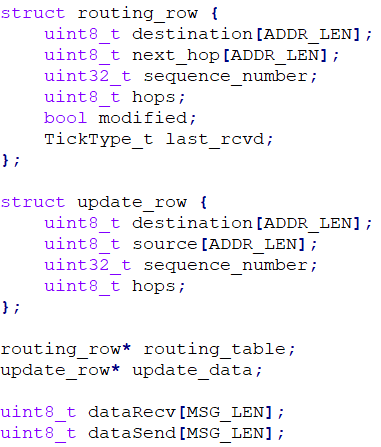
\includegraphics[scale=.5]{structs.png}
\caption{Prikaz programskih struktur za shranjevanje usmerjevalnih podatkov in prometa omrežja.}
\label{g04:structs}
\end{figure}

Dolžina paketov je bila določena kot 32B, in vsebuje štiri vnose po 8B. Vsak izmed vnosov vsebuje najprej 3B, ki predstavljajo naslov ciljne naprave v omrežju. Naslednji 4B vsebujejo sekvenčno številko vnosa v usmerjevalni tabeli. Zadnji bajt pa predstavlja število skokov, ki so potrebni, da iz pošiljatelja paketa dosežemo ciljno napravo.

\subsection{Opravila implementacije}
Implementacija uporablja osem opravil različnih kompleksnosti, ki so tu opisana v naraščajoči prioriteti.
\begin{itemize}
  \item \textbf{DSDV\_init.} Vzpostavi napravo in nRF24L01 modul, določi unikaten naslov naprave (ni implementirano) in inicializira podatkovne tabele. Nato ustvari opravilo nRF24\_listen.
  \item \textbf{nRF24\_listen.} Vsake 200ms preverja, ali je prispelo novo sporočilo. Če je preteklo dovolj časa, ustvari opravilo check\_table in opravilo format\_packet.
  \item \textbf{parse\_packet.} Prebere prispeli paket v polju dataRecv in podatke ustrezno prepiše v posodobitveno tabelo. Nato ustvari opravilo update\_table.
  \item \textbf{check\_table.} Preveri vnose v tabeli in tiste, ki so neaktivni, bodisi označi kot neveljavne (število skokov poveča na maksimalno vrednost) ali pa jih odstrani.
  \item \textbf{update\_table.} Iterira čez vnose v posodobitveni tabeli in nova ciljna vozlišča dodaja v usmerjevalno tabelo. Za obstoječa ciljna vozlišča preverja sekvenčno številko in usmerjevalno tabelo ustrezno spreminja.
  \item \textbf{format\_packet.} Najprej preveri, če je potrebno poslati več kot 4 vrstice ali pa je preteklo dovolj časa od zadnjega oddajanja celotne usmerjevalne tabele, in v tem primeru ustvari opravilo full\_table\_dump. Drugače spremenjene vrstice zapiše v polje dataSend in ustvari opravilo nRF24\_transmit.
  \item \textbf{full\_table\_dump.} Iterira čez usmerjevalno tabelo, vrstice prepisuje v polje dataSend in vmes sinhrono kliče nRF24\_transmit.
  \item \textbf{nRF24\_transmit.} Preneha poslušanje na modulu nRF24L01 in odda paket v polju dataSend.
\end{itemize}

\subsection{Uporabniške nastavitve}
Na vrhu programske implementacije so posebej določene nastavitve, ki jih lahko uporabnik enostavno prilagaja svojim potrebam. Te so:
\begin{itemize}
  \item \textbf{channel.} Kanal omrežja, ki ga naprave uporabljajo.
  \item \textbf{network\_address.} Naslov omrežja, na katerem poslušajo vse naprave.
  \item \textbf{TABLE\_SIZE\_INIT.} Število vrstic v usmerjevalni tabeli ob začetku delovanja.
  \item \textbf{BRCST\_INTERVAL.} Število sekund med oddajanjem sprememb v usmerjevalni tabeli.
  \item \textbf{DUMP\_INTERVAL.} Število sekund med oddajanjem celotne usmerjevalne tabele.
  \item \textbf{CHECK\_INTERVAL.} Število sekund med preverjanjem usmerjevalne tabele za neveljavne povezave.
  \item \textbf{TIMEOUT.} Število sekund od zadnjega prejema po katerih je vnos v usmerjevalni tabeli razumljen kot neveljaven.
  \item \textbf{ENTRY\_DELETE.} Število sekund od zadnjega prejema po katerih se vnos v usmerjevalni tabeli odstrani.
\end{itemize}

\section{Eksperimenti in rezultati}
Za preverjanje pravilnosti delovanje je študentu žal zmanjkalo časa. Program se pravilno prevede s priloženim Makefile. Namen je bil napisati še testni program, ki na eni ploščici preverja pravilno pretvarjanje podatkov v pakete, in iz paketov v vrstice usmerjevalne tabele. Hkrati bi s pritiski na gumb lahko simulirali prispete pakete in preverjali, ali naprava usmerjevalno tabelo pravilno posodobi. Če bo možno, bo testni program spisan do predstavitve, nakar bodo predstavljeni morebitni popravki k implementaciji DSDV in demonstracija delovanja.

\section{Zaključek}
V tem poročilu je bila predstavljena širša tematika področja MANET omrežij, pregled nekaterih rešitev k problemu usmerjanja prometa v le-teh, in splošen opis usmerjevalnega algoritma DSDV. Nato so bile na kratko predstavljene še podrobnosti modula nRF24L01 pred obsežnejšim opisom programske implementacije algoritma.

Za modul nRF24L01 je bila v sklopu projekta uspešno pripravljena implementacija DSDV algoritma, ki zajema njegovo osnovno delovanje. Spisan program omogoča zaznavanje bližnjih naprav, obveščanje bližnjih naprav o lastni prisotnosti, in ustrezno popravljanje usmerjevalne tabele glede na pridobljene podatke.

Ker pravilno delovanje implementacije ni bilo preverjeno, bi se nadaljnje delo moralo najprej fokusirati na odpravljanje morebitnih napak. V implementaciji manjka tudi pravilno pridobivanje specifičnega naslova naprave, ki je bil v programu nastavljen na fiksno vrednost.

Poleg tega manjka implementacija funkcionalnosti usmerjanja. Program bi moral biti sposoben prejeti paket, ki je naslovljen na specifično napravo, in ga glede na podatke v usmerjevalni tabeli pravilno posredovati naprej. Naprava s trenutno implementacijo ne posluša sporočil, ki so naslovljena točno nanjo namesto na omrežje nasploh.

Poleg teh dopolnitev obstajajo še tri možnosti za dodatno nadgradnjo. Prvič je možno, da sekvenčne številke vrstic v tabelo presežejo maksimalno vrednost. V trenutni implementaciji s povečanjem vsakih 5 sekund in uporabe 4B sekvenčne številke, bi za to porabili približno 340 let, kar je nerealno. Če pa bi se presežek maksimalne vrednosti rešil programsko, bi se lahko zmanjšala velikost sekvenčne številke, kar bi omogočalo uporabo daljših naslovov naprav oz. pošiljanje več vrstic usmerjevalne tabele v enem paketu.

Druga dopolnitev je zavarovanje naprav. Zaradi varnostnih pomanjkljivosti, ki so bile izpostavljene v uvodu poročila, bi bilo smiselno implementirati nadgradnjo algoritma, ki implementacijo ustrezno zavaruje. Nenazadnje pa bi bilo smiselno tudi preveriti optimalnost delovanja ob različnih primerih delovanja glede na različne topologije omrežja in uporabniške nastavitve implementacije. S tem bi lahko dosegli veliko boljše delovanje implementacije za različne potrebe.


